\subsection{Technical parameters}
The frist set of indicators are technical parameters that define the performance of each reactor design form an engineering standpoint.
An overview of technical parameters is presented in Table \ref{tab:indicators-technical}.

\textbf{Thermal efficiency} indicates the fraction of thermal power generated by fission that is converted into net electrical power, accounting for in-plant consumption. Efficiency values were calculated using net electrical power output and thermal power data from the \gls{aris} database \cite{iaea2025aris}:
$$
\eta = \frac{P_{el,net}}{P_{th}}
$$
This indicator is a way to judge the thermal-hydraulic design of the reactor.

\textbf{Discharge Burnup} measures the energy extracted per unit of heavy metal from the nuclear fuel ($MWd/tonHM$). Data for APR1400 and AP1000 were sourced from the \gls{aris} database \cite{iaea2025aris}, while EPR 1750 data were obtained from \cite{NRC_ML052280170}. Ranges are provided for SMRs due to design variability. Such value is indicative of the neutronics and core design of the reactor.


\textbf{Net Power Output} has to be considered when choosing a power plant in relation to the needs of the local energy market, for instance a country that is constantly importing a substantial amount of energy might prefer large power plants rather then \glspl{smr}, on the other hand countries where renewable energy dominates the mix, small and flexible power could be preferred. For three large reactors data was sourced from \cite{IAEA_PRIS_2025} while for \glspl{smr} data was obtained from \cite{iaea2025aris}.


\textbf{\glspl{lfc}} can be quantitatively assessed using characteristic curves that represent ramp-up and ramp-down rates as a function of load (expressed as percentage of nominal power $\%P_{nom}$), as illustrated in Figure \ref{fig:load-following-curve}. To facilitate comparative analysis, these performance curves are reduced to scalar values through integration of the area under said curve.

\begin{figure}[!hb]
    \centering
    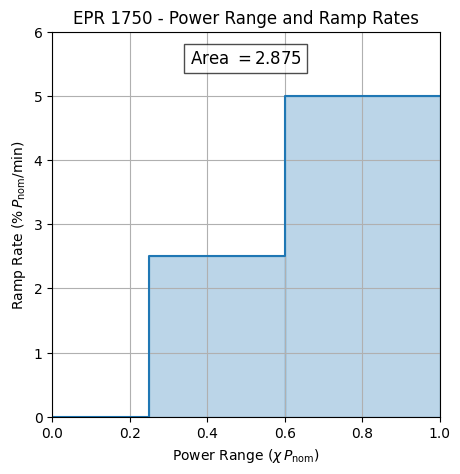
\includegraphics[width=0.7\textwidth]{imgs/load_following_curve.png}
    \caption{Example \gls{lfc} curve for EPR-1750}
    \label{fig:load-following-curve}
\end{figure}

For benchmarking purposes, the \gls{lfc} of a pair a tipical gas powered plant was computed. Specifically, a combined cyle plant featuring two heavy-duty \gls{ge} 9HA.02 gas turbines (2015 data) \cite{GE_9HA_Gas_Turbine_2015}. 
Sources for load following data for APR1400, AP1000, BWRX-300 and Rolls Royce SMR where sourced from \cite{iaea2025aris}, while EPR 1750 data was obtained from \cite{OECD_NEA_Load_Following_2011}. For NuScale data was sourced from \cite{ENCO_SMR_Analysis_2022}.

\begin{table}[!ht]
    \centering
    \begin{tabularx}{0.6\textwidth}{l X X}
        \toprule
        \textbf{Reactor Model} & \textbf{S1} & \textbf{S2}\\
        \midrule
        APR1400           & 1340 & 0.21 \\
        EPR 1750          & 1630 & 2.88 \\
        AP1000            & 1120 & 4.25 \\
        BWRX-300          & 300 & 0.25 \\
        Rolls Royce SMR   & 470 & 2.00 \\
        NuScale (Voygr-6) & 462  & 2.00 \\
        \gls{ge} 9HA.02 2xCC    & 1515 & 7.02 \\
        \bottomrule
    \end{tabularx}
    \caption{System Indicators: S1: Net Electric Power Output [$MW_{e,net}$], S2: \gls{lfc} [$\%P_{nom}/min$]}
    \label{tab:indicators-system}
\end{table}